\documentclass[preview]{standalone}

\usepackage{amsmath}
\usepackage{amssymb}
\usepackage{stellar}
\usepackage{definitions}
\usepackage{bettelini}
\usepackage{tikz}

\begin{document}

\id{graph-trees}
\genpage

\section{Trees}

\begin{snippetdefinition}{tree-definition}{Tree}
    A \emph{tree} is a connected \graph with no cycles.
\end{snippetdefinition}

\begin{snippet}{tree-nontree-illustration}
    The graph on the left is a tree; the graph on the right is not a tree
    because it contains cycles.
    \[
        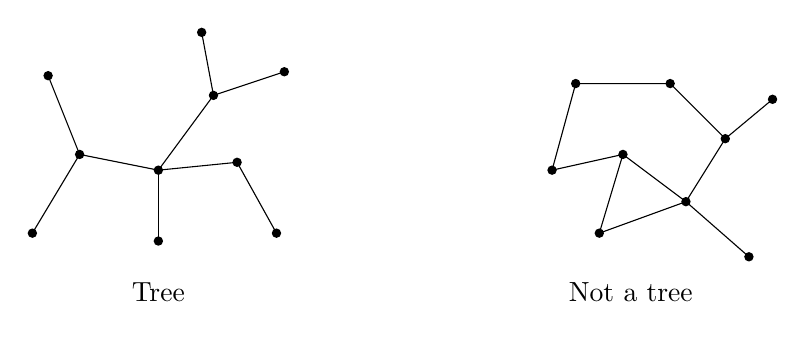
\begin{tikzpicture}[scale=1]
            \begin{scope}
                \node at (0,-1.55) {Tree};

                \coordinate (a) at (0,0);
                \coordinate (b) at (-1,0.2);
                \coordinate (c) at (-1.4,1.2);
                \coordinate (d) at (-1.6,-0.8);
                \coordinate (e) at (0,-0.9);
                \coordinate (f) at (1,0.1);
                \coordinate (g) at (1.5,-0.8);
                \coordinate (h) at (0.7,0.95);
                \coordinate (i) at (1.6,1.25);
                \coordinate (j) at (0.55,1.75);

                \draw (a)--(b)--(c);
                \draw (b)--(d);
                \draw (a)--(e);
                \draw (a)--(f)--(g);
                \draw (a)--(h)--(i);
                \draw (h)--(j);

                \foreach \p in {a,b,c,d,e,f,g,h,i,j}{
                    \fill (\p) circle (1.7pt);
                }
            \end{scope}

            \begin{scope}[xshift=6cm]
                \node at (0,-1.55) {Not a tree};

                \coordinate (a) at (-1,0);
                \coordinate (b) at (-0.7,1.1);
                \coordinate (c) at (0.5,1.1);
                \coordinate (d) at (1.2,0.4);
                \coordinate (e) at (0.7,-0.4);
                \coordinate (f) at (-0.1,0.2);
                \coordinate (g) at (-0.4,-0.8);
                \coordinate (h) at (1.8,0.9);
                \coordinate (i) at (1.5,-1.1);

                \draw (a)--(b)--(c)--(d)--(e)--(f)--(a);
                \draw (f)--(g)--(e);
                \draw (d)--(h);
                \draw (e)--(i);

                \foreach \p in {a,b,c,d,e,f,g,h,i}{
                    \fill (\p) circle (1.7pt);
                }
            \end{scope}
        \end{tikzpicture}
    \]
\end{snippet}

\begin{snippet}{trees-are-simple}
    Every tree is a simple graph. Indeed, a loop is a cycle of length \(1\),
    and two parallel edges form a cycle of length \(2\).
\end{snippet}

\begin{snippetproposition}{finite-simple-graph-edge-count-proposition}{Finite simple graphs have finitely many edges}
    Let \(G\) be a simple \graph with \(n\) vertices, where \(n\in\integers^+\).
    Then \(G\) has at most
    \[
        \binom{n}{2}=\frac{n(n-1)}{2}
    \]
    edges. In particular, \(G\) has finitely many edges.
\end{snippetproposition}

\begin{snippetproof}{finite-simple-graph-edge-count-proof}{finite-simple-graph-edge-count-proposition}{Finite simple graphs have finitely many edges}
    Since \(G\) is simple, there is at most one edge between any two distinct
    vertices, and there are no loops. Hence every edge is determined by an
    unordered pair of distinct vertices. The number of such pairs is
    \[
        \binom{n}{2}=\frac{n(n-1)}{2}.
    \]
\end{snippetproof}

\begin{snippetcorollary}{finite-tree-has-finite-edges-corollary}{Finite trees have finitely many edges}
    Every tree with finitely many vertices has finitely many edges.
\end{snippetcorollary}

\begin{snippetproof}{finite-tree-has-finite-edges-proof}{finite-tree-has-finite-edges-corollary}{Finite trees have finitely many edges}
    Every tree is simple, so the result follows from the edge bound for finite
    simple graphs.
\end{snippetproof}

\begin{snippetdefinition}{leaf-definition}{Leaf}
    Let \(G\) be a \graph.
    A vertex of degree \(1\) is called a \emph{leaf}.
\end{snippetdefinition}

\begin{snippetproposition}{finite-tree-leaves-proposition}{Leaves in a finite tree}
    Let \(T\) be a finite tree with at least two vertices.
    Then \(T\) has at least two leaves.
\end{snippetproposition}

\begin{snippetproof}{finite-tree-leaves-proof}{finite-tree-leaves-proposition}{Leaves in a finite tree}
    Choose a path of maximum possible length in \(T\):
    \[
        v_0,v_1,\ldots,v_k.
    \]
    We show that \(v_0\) and \(v_k\) are leaves.

    Suppose, for instance, that \(v_0\) has a neighbor \(w\neq v_1\).
    If \(w\) is not on the path, then
    \[
        w,v_0,v_1,\ldots,v_k
    \]
    is a longer path, contradicting maximality. If \(w\) is already on the
    path, then \(w\) together with the segment of the path from \(w\) to
    \(v_0\) forms a cycle, impossible in a tree.

    Thus \(v_0\) has \(v_1\) as its only neighbor, so it has degree \(1\).
    The same argument applies to \(v_k\).
\end{snippetproof}

\begin{snippettheorem}{finite-tree-edge-characterization-theorem}{Finite trees and the number of edges}
    Let \(G\) be a finite connected \graph with \(n\) vertices.
    Then \(G\) is a tree \ifandonlyif \(G\) has \(n-1\) edges.
\end{snippettheorem}

\begin{snippetproof}{finite-tree-edge-characterization-proof}{finite-tree-edge-characterization-theorem}{Finite trees and the number of edges}
    \begin{iffproof}
        \item Suppose that \(G\) is a tree. We prove by induction on \(n\) that
        \(G\) has \(n-1\) edges.

        If \(n=1\), then \(G\) has no edges, so it has \(0=n-1\) edges.

        Let \(n>1\). By the leaf proposition, \(G\) has a leaf \(v\). Let \(e\)
        be the unique edge incident with \(v\), and let \(G'\) be obtained from
        \(G\) by deleting \(v\) and \(e\).

        The graph \(G'\) contains no cycle, because any cycle in \(G'\) would
        also be a cycle in \(G\). It is also connected: if \(u,w\in V(G')\),
        any path from \(u\) to \(w\) in \(G\) cannot pass through the leaf \(v\)
        as an internal vertex. Hence that path lies entirely in \(G'\).

        Thus \(G'\) is a tree with \(n-1\) vertices. By the induction
        hypothesis, \(G'\) has \(n-2\) edges. Adding back the edge \(e\), the
        graph \(G\) has \(n-1\) edges.

        \item Suppose that \(G\) is connected with \(n\) vertices and \(n-1\)
        edges. We show that \(G\) contains no cycle.

        If \(G\) contained a cycle, deleting one edge of that cycle would leave
        the graph connected, because the endpoints of the deleted edge would
        still be joined by the rest of the cycle. If another cycle remained,
        repeat the procedure.

        Since the graph is finite, after finitely many steps we obtain a
        connected graph \(T\) with no cycles, hence a tree, with the same
        \(n\) vertices and fewer than \(n-1\) edges. This is impossible by the
        first implication, because every tree with \(n\) vertices has exactly
        \(n-1\) edges.

        Therefore \(G\) has no cycles. Since \(G\) is connected, it is a tree.
    \end{iffproof}
\end{snippetproof}

\begin{snippetproposition}{tree-unique-paths-proposition}{Unique paths in trees}
    A \graph \(G\) is a tree \ifandonlyif for every pair of distinct vertices
    \(u,v\in V(G)\), there exists a unique path joining \(u\) and \(v\).
\end{snippetproposition}

\begin{snippetproof}{tree-unique-paths-proof}{tree-unique-paths-proposition}{Unique paths in trees}
    \begin{iffproof}
        \item Suppose that \(G\) is a tree. Since \(G\) is connected, every two
        distinct vertices are joined by at least one path. If there were two
        distinct paths from \(u\) to \(v\), following one path from \(u\) to
        \(v\) and the other back from \(v\) to \(u\) would produce a closed
        walk. Removing repetitions from this closed walk yields a cycle,
        impossible in a tree.

        \item Conversely, suppose that every pair of distinct vertices is
        joined by a unique path. Then \(G\) is connected. Moreover, \(G\)
        cannot contain a cycle, because two distinct vertices on a cycle can be
        joined by following the cycle in two different directions. Hence \(G\)
        is connected and has no cycles, so it is a tree.
    \end{iffproof}
\end{snippetproof}

\section{Counting small trees}

\begin{snippetexercise}{small-labeled-trees-exercise}{Small labelled trees}
    Let the vertex set be \(\{1,2,\ldots,n\}\). How many trees exist with this
    vertex set?

    For the first values of \(n\), one obtains:
    \[
        \begin{array}{c|c}
            n & \text{number of labelled trees} \\
            \hline
            1 & 1 \\
            2 & 1 \\
            3 & 3
        \end{array}
    \]
    For \(n=3\), the possible labelled trees are
    \[
        \begin{tikzpicture}[scale=0.9,baseline={(current bounding box.center)}]
            \begin{scope}
                \coordinate (a) at (0,0);
                \coordinate (b) at (1,0);
                \coordinate (c) at (2,0);
                \draw (a)--(b)--(c);
                \foreach \p/\lab in {a/1,b/2,c/3}{
                    \fill (\p) circle (1.6pt);
                    \node[above] at (\p) {\(\lab\)};
                }
            \end{scope}

            \begin{scope}[xshift=4cm]
                \coordinate (a) at (0,0);
                \coordinate (b) at (1,0);
                \coordinate (c) at (2,0);
                \draw (a)--(b)--(c);
                \foreach \p/\lab in {a/1,b/3,c/2}{
                    \fill (\p) circle (1.6pt);
                    \node[above] at (\p) {\(\lab\)};
                }
            \end{scope}

            \begin{scope}[xshift=8cm]
                \coordinate (a) at (0,0);
                \coordinate (b) at (1,0.5);
                \coordinate (c) at (1,-0.5);
                \draw (a)--(b);
                \draw (a)--(c);
                \foreach \p/\lab in {a/1,b/2,c/3}{
                    \fill (\p) circle (1.6pt);
                    \node[above] at (\p) {\(\lab\)};
                }
            \end{scope}
        \end{tikzpicture}
    \]
    These three trees are isomorphic as unlabelled graphs, but they are
    distinct as labelled trees.
\end{snippetexercise}

\begin{snippetexercise}{four-vertex-labelled-trees-exercise}{The case of four labelled vertices}
    Prove that the number of labelled trees with vertex set \(\{1,2,3,4\}\)
    is \(16\).

    This is the first non-trivial case of Cayley's formula:
    \[
        n^{n-2}=4^2=16.
    \]
\end{snippetexercise}

\end{document}
